\begin{figure}[t]
    \centering
    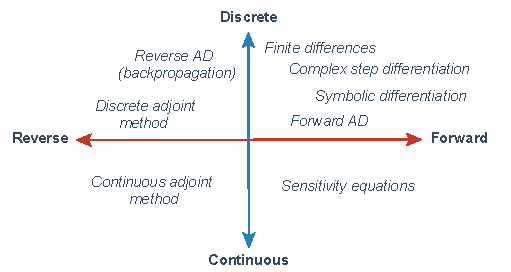
\includegraphics[width=0.80\textwidth]{figures/scheme-methods.pdf}
    \caption{Schematic representation of the different methods available for differentiation involving differential equation solutions. These can be classified depending if they find the gradient by solving a new system of differential equations (\textit{continuous}) or if instead they manipulate unit algebraic operations (\textit{discrete}). Additionally, these methods can be categorized based on their alignment with the direction of the numerical solver. If they operate in the same direction as the solver, they are referred to as \textit{forward methods}. Conversely, if they function in the opposite direction, they are known as \textit{reverse methods}.}
    \label{fig:scheme-all-methods}
\end{figure}

There is a large family of methods for computing gradients and sensitivities of systems of differential equations. 
Depending on the number of parameters and the complexity of the differential equation we are trying to solve, they have different mathematical, numerical, and computational advantages.
These methods can be roughly classified as  follows\cite{ma2021comparison}. 
\begin{itemize}
    \item \textit{Continuous} vs \textit{discrete}  methods
    \item \textit{Forward} vs \textit{reverse} methods
\end{itemize}
Figure \ref{fig:scheme-all-methods} displays a classification of some methods under this two-fold classification. 

The \textit{continuous} vs \textit{discrete} difference is one of mathematical nature. 
When solving for the gradient of a differential equation, one needs to derive both a mathematical expression for the gradient (the \textit{differentiation step}) and solve the equations using a numerical solver (the \textit{discretization step})\cite{bradley2013pde, Onken_Ruthotto_2020, FATODE2014, Sirkes_Tziperman_1997}. 
Depending on the order of these two operations, we are going to talk about discrete methods (discretize-differentiate) or continuous methods (differentiate-discretize). 
In the case of \textit{discrete} methods, gradients are computed based on simple function evaluations of the solutions of the numerical solver (finite differences, complex step differentiation) or by manipulation of atomic operations inside a numerical solver (AD, symbolic differentiation, discrete adjoint method). 
In the case of \textit{continuous} methods, a new set of differential equations is derived for the sensitivity (sensitivity equations) or the adjoint (continuous adjoint method) of the system, both quantities that allow the calculation of the desired gradient.   
% We can either discretize the original system of ODEs in order to numerically solve it and then find an strategy to differentiate it; or instead define new equations for the differentiation step and later numerically solver them.
When comparing between discrete and continuous methods, more than talking about computational efficiency we are focusing on the mathematical consistency of the method, that is, \textit{is the method estimating the right gradient?}. 
When using discrete methods, we may have a method that is algorithmically correct, meaning that is computing the gradient of the solver discretization, but is not really approximating the gradient of the true solution of the differential equation. 

The \textit{forward} vs \textit{backward} distinction regards when the gradient is computed, if this happens during the forward pass of the numerical solver or in a later recalculation \cite{Griewank:2008kh}. 
In all \textit{forward} methods the solution of the differential equation is solved sequentially and simultaneously with the gradient during the forward pass of the numerical solver.  
On the contrary, \textit{reverse} methods compute the gradient tracking backwards the forward model by resolving a new problem that moves in the opposite direction as the original numerical solver 
For systems of ODEs and initial value problems (IVPs), most numerical methods solve the differential equation progressively moving forward in time, reason why forward methods solve the gradient moving \textit{forward} in time - or, instead, they solve a new system that goes \textit{backwards} in time.

As we will discuss in the following section, forward methods are very efficient for problems with a small number of parameters we want to differentiate with respect to, while backwards methods are more efficient for a large number of parameters  but they came with a larger memory cost which needs to be overcome using different performance tricks. 
With the exception of finite differences and complex step differentiation, the rest of the forward methods (i.e. forward AD, sensitivity equations, symbolic differentiation) compute the full sensitivity of the differential equation, that is, how the full solution of the ODEs changes when we change the parameters of the model. 
% \todo[inline]{Last sentence is also a bit vague: indeed, the forward method computes the impact of changes of the input on all outputs, but it only ever computes a directional derivative (i.e., in the direction of the input perturbation); that's an important distinction. Or I misunderstood something?}
This can be computationally expensive for large systems. 
Conversely, reverse methods are based in the computation of intermediate variables, known as the adjoint or dual variables, that cleverly avoid the unnecessary calculation of the full sensitivity at expenses of larger memory cost \cite{Givoli_2021}. 
For this reason backward methods can be also labeled as adjoint methods \cite{ma2021comparison}. 

One extra distinction between methods is with regards to how computationally entangled the numerical solver and the differentiation machinery are. 
With the exception of the discrete adjoint methods, this coincides with discrete-continuous classification. 
However, the construction of the discrete adjoint (which surprisingly is one of the most popular in the literature) is based on the numerical solver, something that does not happen with the other discrete methods. 
While this might not have big conceptual implications, it is an important consideration when using software that integrates numerical solvers and differentiation, a distinction that will help in the discussion in Section \ref{sec:computational-implementation}.

% It is important to note that if all the methods we explore in this section are mathematically correct, \textit{that does not imply they are numerically stable}.
% These statements applied to methods based on pure automatic differentiation as well as adjoint methods. 
% We explore this consideration in more detail in section \ref{sec:computational-implementation}.

The rest of this section is organized as follows. 
We will first introduce some basic mathematical notions that are going to facilitate the discussion of the sensitivity methods (Section \ref{section:preliminaries}).
Then we will embark in the mission of mathematically introducing each one of methods listed in Figure \ref{fig:scheme-all-methods}.
We will finalize the discussion in Section \ref{section:compatison-math} with an comparison of some of mathematical foundations of these methods. 
% More specificlacy, our goal here is try to enlight the closed resamblance of the methods 